%%%%%%%%%%%%%%%%%%%%%%%%%%%%%%%%%%%%%%%%%
% Simple Sectioned Essay Template
% LaTeX Template
%
% This template has been downloaded from:
% http://www.latextemplates.com
%
% Note:
% The \lipsum[#] commands throughout this template generate dummy text
% to fill the template out. These commands should all be removed when
% writing essay content.
%
%%%%%%%%%%%%%%%%%%%%%%%%%%%%%%%%%%%%%%%%%

%----------------------------------------------------------------------------------------
%	PACKAGES AND OTHER DOCUMENT CONFIGURATIONS
%----------------------------------------------------------------------------------------

\documentclass[12pt]{article} % Default font size is 12pt, it can be changed here

\usepackage{geometry} % Required to change the page size to A4
\geometry{a4paper} % Set the page size to be A4 as opposed to the default US Letter

\usepackage{graphicx} % Required for including pictures

\usepackage{float} % Allows putting an [H] in \begin{figure} to specify the exact location of the figure
\usepackage{wrapfig} % Allows in-line images such as the example fish picture

\usepackage{lipsum} % Used for inserting dummy 'Lorem ipsum' text into the template

\usepackage{multicol}
\usepackage{amsmath}

\usepackage[utf8x]{inputenc}
\usepackage{amsfonts,euscript,latexsym,amssymb}
\usepackage[portuguese,USenglish]{babel}

\linespread{1.2} % Line spacing

%\setlength\parindent{0pt} % Uncomment to remove all indentation from paragraphs

\graphicspath{{Pictures/}} % Specifies the directory where pictures are stored

\begin{document}

%----------------------------------------------------------------------------------------
%	TITLE PAGE
%----------------------------------------------------------------------------------------

\begin{titlepage}

\newcommand{\HRule}{\rule{\linewidth}{0.5mm}} % Defines a new command for the horizontal lines, change thickness here

\center % Center everything on the page

\textsc{\LARGE Instituto Superior Tecnico}\\[1cm] % Name of your university/college
\textsc{\Large Programação de Sistemas}\\[0.5cm] % Major heading such as course name
\textsc{\large}\\[0.5cm] % Minor heading such as course title
\HRule \\[0.4cm]
{ \LARGE \bfseries Key-Value Store}\\[0.4cm]
% Title of your document
\HRule \\[1cm]

\begin{minipage}{0.6\textwidth}
\begin{flushleft} \large
\emph{Autores:}\\
73640 - André \textsc{Stielau}\\
73198 - João \textsc{Almeida}\\

\end{flushleft}
\end{minipage}
~
\\[1cm]
{\large 29 de Maio de 2016}\\[1cm] % Date, change the \today to a set date if you want to be precise

\begin{figure}[H]
\centering

\includegraphics[width=0.7\textwidth]{./Pictures/tecnico.png}
\end{figure}

\vfill % Fill the rest of the page with whitespace

\end{titlepage}

%----------------------------------------------------------------------------------------
%	TABLE OF CONTENTS
%----------------------------------------------------------------------------------------

%\tableofcontents % Include a table of contents

%\newpage % Begins the essay on a new page instead of on the same page as the table of contents

%----------------------------------------------------------------------------------------
%	INTRODUCTION
%----------------------------------------------------------------------------------------

\iffalse

O relatório deverá conter a seguinte informação

Esquema dos componentes e suas ligações
Detalhes de implementação de cada um dos componentes
Detalhes dos modelos de comunicação entre componentes (funcionalidade e protocolos)

Na descrição dos componentes é necessário referir explicitamente o seguinte

Estrutura de dados que armazena os pares (chave, valor)
Mecanismos de sincronização no acesso à estrutura de dados
Mecanismo de gestão da Threads
Protocolo de tolerância à falta
Protocolo de backup/recuperação dos dados
Tratamento de erros
\fi

\section{System overview}
\label{sec:Systemoverview}



\begin{figure}[H]
\centering
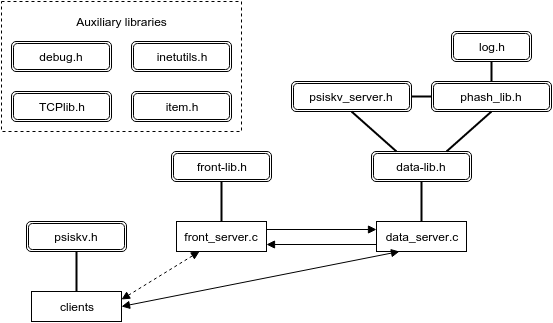
\includegraphics[width=0.8\textwidth]{./Pictures/KV_SystemOverview.png}
\caption{Overview of the system components and libraries}\label{fig:KVSyst}
\end{figure}

Figure \ref{fig:KVSyst} shows an overview of how the most important libraries and components of the system are connected.

\section{Key Value Data Structure}

The \textbf{data storage} is implemented on an \textbf{hash table} where each bucket of the hash table is a \textbf{linked list} and each list entry holds the key and a pointer to the value. See Figure~\ref{fig:DataOverview} for more details.

\begin{figure}[H]
\centering
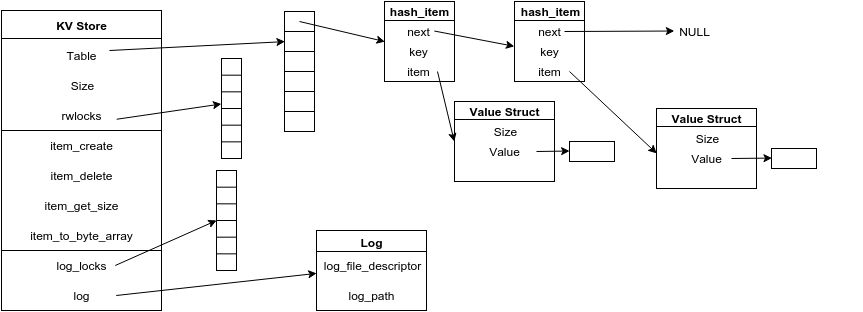
\includegraphics[width=\textwidth]{./Pictures/DataStructures.png}
\caption{Overview of Data Structures}\label{fig:DataOverview}
\end{figure}

The hash table component is implemented with \textbf{data abstraction} in mind, in this system it holds a byte array and its size, but could be used to store any kind of data. The item to be stored on the hash table is implemented in  another component, in the key-value store case to the \emph{psiskv\_server.h}. There all necessary auxiliary functions are implemented and a pointer to them is stored on the data structure.

\subsection{Backup and Log}
\label{sub:BackupLog}

To maintain data between data server executions a backup and a log file are used. The backup stores a snapshot of the state of the Hash table, while the log stores all successful write and delete commands made since startup.

At startup the data server initializes the hash table according to the flowchart on figure~\ref{fig:BackupLogFlow}.

\begin{figure}[H]
\centering
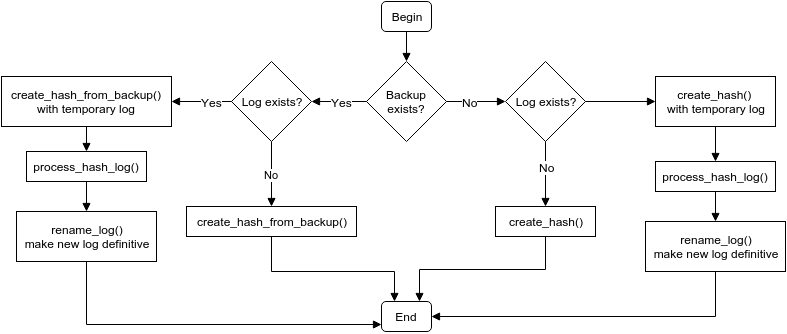
\includegraphics[width=\textwidth]{./Pictures/BackupLogFlow.png}
\caption{Data server hash table initialization flow}\label{fig:BackupLogFlow}
\end{figure}

At a clean exit the data server creates a new backup and deletes the log file. Which means that there only exists a log file if the data server didn't exit orderly.

To prevent data consistency problems the backup file is only deleted after a new backup file is ready.



\subsection{Synchronization}
\label{sub:Synchronization}

To guarantee data consistency on the hash table and on the log file a set of measures


\section{Key-Value Communication}

To use the Key-Value Store the client uses the \emph{psiskv.h} library to establish a connection and make requests.
The communication flow is exemplified on figure~\ref{fig:Comms}. During the \textbf{kv\_connect} the \textbf{client} connects to the \textbf{Front Server} which responds with the port of the \textbf{Data Server} and then the client connects to it and is ready to make requests.

\begin{figure}[H]
\centering
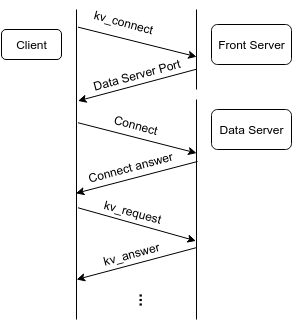
\includegraphics[width=0.6\textwidth]{./Pictures/CommunicationFlow.png}
\caption{Overview of the client KV store communication flow}\label{fig:Comms}
\end{figure}

The structure of the messages exchanged between the \textbf{client} and the \textbf{Data server} is:  a  enumerate \emph{msg\_type}, a \emph{uint32\_t} with the \textbf{key} and an \emph{unsigned int} with the length of the value. The possible message types are:
\begin{description}
    \item[WRITE\_REQ] - write request;
    \item[WRITE\_REQ\_OW] - write request with overwrite;
    \item[WRITE\_RESP] - write response;
    \item[READ\_REQ] - read request;
    \item[READ\_RESP] - read response;
    \item[DELETE\_REQ] - delete request;
    \item[DELETE\_RESP] - delete response;
    \item[ERROR] - error message;
\end{description}
After a \emph{WRITE\_REQ} or a \emph{READ\_RESP} a buffer containing the value to store is transmitted over TCP with the length being specified on the previous message.


\subsection{Error Messages}
\label{sub:ErrorMessages}

\section{Inter Server Communication}
\label{sec:CommunicationProtocol}
To ensure that the processes keep each other alive, the data server knows when to shutdown and the front server knows the Data Server's address, the servers have a communication protocol.
One thread in each server, called 'communication worker', exchange the following messages:
  \begin{description}
    \item[PING] - default message, just to ensure the other process is still alive, 1 per second;
    \item['PORT'] - informs the Front Server about the Data Server's port;
    \item[EXIT] - commands the Data Server to shut down;
    \item[OK] - informs the Front Server that the Data Server received the EXIT command;
  \end{description}


\section{Front Server}
\label{sec:FrontServer}

\begin{figure}[H]
\centering
\includegraphics[width=0.7\textwidth]{./Pictures/Communications-Front.png}
\caption{All communications with Front Server}\label{fig:CommunicationsFront}
\end{figure}

\section{Data Server}
\label{sec:DataServer}

\begin{figure}[H]
\centering
\includegraphics[width=0.7\textwidth]{./Pictures/Communications-Data.png}
\caption{All communications with Data Server}\label{fig:CommunicationsData}
\end{figure}

\subsection{Thread Management}
\label{sub:ThreadManagement}

The threads are created following the \textbf{on demand} strategy for both the front and the data server.

On the front server there are three threads always running and others created to handle kv_connect requests. There is one thread reading from stdin to check if the user tells the server to quit, there is the main thread, locked in a accept for the TCP socket that creates new threads for each new request and the communication socket, that exchanges messages with the data server, see section \ref{sec:CommunicationProtocol}.

On the 

\section{Fault Tolerance}
\label{sec:FaultTolerance}

\section{Clients}
\label{sec:Clients}








\end{document}
